
\section{Probability Theory}
%\renewcommand{\baselinestretch}{1.25}\normalsize
    \subsection{Combinatorics}
        \begin{minipage}{13.5cm}
        \begin{tabular}{| p{5.5cm} | c | c |}
            \hline
            Type of selection or composition of $k$ from $n$ elements    & \multicolumn{2}{c|}{Number of possibilities}\\
             & without repetitions        & with repetitions\\
             & $(k\leq n)$                & $(k\leq n)$ \\
             \hline
            Permutations & $P_n=n!(n=k)$ &
            $P_n^{(k)}=\frac{n!}{k!}$ \\ & &\\
            Combinations & $C_n^{(k)}=\binom n k$ &
            $C_n^{(k)}=\binom{n+k-1} k$\\
            & &\\
            Variations & $V_n^{(k)}=k!\binom n k$ & $V_n^{(k)}=n^k$\\
            \hline
        \end{tabular}
        \end{minipage}
        \begin{minipage}{5cm}
        $\binom n k$ with TR: \texttt{nCr(n,k)} \hspace{9.3mm}En\\
        \hspace*{19mm} \texttt{Kombinat(n,k)} De
        \end{minipage}
        \begin{list}{$\bullet$}{\setlength{\itemsep}{0cm} \setlength{\parsep}{0cm} \setlength{\topsep}{0.1cm}} 
            \item \textbf{Permutations}: Given are $n$ different objects. Then there are $n!$
            different orders in which these objects can be arranged. \\
            e.g.: $x,y,z;\quad x,z,y;\quad z,y,x;\ldots$
         % \item Permutation is called an arrangement of $n$ elements in a certain
        %       order
            \item \textbf{Combination}: Given are $n$ different objects. Then there are $\binom n k$
            ways to select $k$ objects from them, if the order does not matter. \\
            e.g.: How many different ways are there to select 6 numbers out of 49
            in the lottery?
         % \item Combination is called a selection of $k$ elements from $n$ elements
         %       without considering the order
            \item \textbf{Variation} is called a selection of $k$ elements from $n$
                different elements considering the order
        \end{list}


\vspace{5mm}
    \begin{minipage}{6.8cm}
    \subsection{Probability}
        \begin{tabular}{ll}
            Range of values:
            & ${0}\le{P(A)}\le{1}$\\ \\
            Certain event:
            & $P(\Omega)=1$\\ \\
            Impossible event:
            & $P(\emptyset)=0$
        \end{tabular}
    \end{minipage}
        \begin{minipage}{11.2cm}
        \textbf{Calculation rules}\\
            \begin{tabular}{ll}
                Complementary event:
                &$P(\bar{A})=P({\Omega}\setminus{A})=1-P(A)$\\ \\
                Difference of the events A and B:
                &$P({A}\setminus{B})=P(A)-P({A}\cap{B})$\\ \\
                Union of two events:
                &$P({A}\cup{B})=P(A)+P(B)-P({A}\cap{B})$
            \end{tabular}
        \end{minipage}
\vspace{1mm}


	\subsection{Laplace Events}
		In a finite probability space $\Omega$, all
		elementary events have the same probability.
		\begin{center}
		$P(A)=\dfrac{\left| A\right|}{\left|\Omega\right|}$
		\end{center}

	\subsection{Independent Events}
		Independent events $A$ and $B$ are present when:\\
		\hspace*{8mm} $P(A\mid B)=P(A)$ \hspace{4mm} and \hspace{4mm}
		$P(B\mid A)=P(B)$\\
		is satisfied. For them, it applies\\
		\hspace*{8mm} $P(A\cap B)=P(A)P(B)$\\
		The fact that A has occurred has no influence on the 
		probability of B.\vspace{1mm}


	\subsection{Conditional Probability}
		The probability of the occurrence of event $A$ given that
		event $B$ has already occurred.
		\begin{center}
		$P(A\mid B)= \dfrac{P(A\cap B)}{P(B)}=\underbrace{\frac{P(A)\cdot
		P(B)}{P(B)}=P(A)}_{\text{only if independent}}$ 
		\end{center}


	\subsection{Bayes' Theorem}
		\begin{tabular}{ll}
		$P(B\mid A)=P(A\mid B) \cdot\dfrac{P(B)}{P(A)}$\vspace{1mm}
		\end{tabular}


	\subsection{Total Probability}
		\begin{tabular}{ll}
		$P(A)=\sum\limits_{i=1}^N P(A\mid G_i)\cdot P(G_i)$
		\end{tabular}


	\subsection{Probability Distribution}

		\subsubsection{Distribution Function}
			\renewcommand{\arraystretch}{1.5}
			\begin{tabular}[]{|l|l|}
				\hline
				\textbf{discrete} & \textbf{continuous}\\
				\hline
				\hline
				$P(X\leq x)=F(x)=\sum\limits_{k=-\infty}^x p_k$ &
				$P(X\leq x)=F(x)=\int\limits_{-\infty}^x\varphi(\tilde{x})d\tilde{x}$\\
				$P(X>x)=1-P(X\leq x)$ & 
				$P(X>x)=1-P(X\leq x)$\\     
				   
				$P(\alpha_1 \le X \leq \alpha_2)=F(\alpha_2)-F(\alpha_1)=\sum\limits_{k=\alpha_1}^{\alpha_2} p_k$ &          
				$P(\alpha_1 \le X \leq \alpha_2)=F(\alpha_2)-F(\alpha_1)=\int \limits_{\alpha_1}^{\alpha_2}\varphi(\tilde{x})d\tilde{x}$\\
			
				$F_{x_1,x_2}(\alpha_1,\alpha_2)=P(\alpha_1 \le X_1 , \alpha_2\leq X_2)$&
				$F_{x_1,x_2}(\alpha_1,\alpha_2)=P(\alpha_1 \le X_1 , \alpha_2\leq X_2)$\\
				\hline
			\end{tabular}
			\renewcommand{\arraystretch}{1}
	
			\textbf{Properties}
					$$\boxed{\mathbb{D}(F) = \mathbb{R}} \qquad \boxed{\mathbb{W}(F)
					\in[0,1]} \qquad \boxed{F(-\infty)=0} \qquad  \boxed{F(\infty)=1}
					\qquad \boxed{F(x) \text{ is monotonically increasing}}$$
	
	
		\subsubsection{Probability Density }
			\begin{tabular}{p{7.3cm}p{8.5cm}}
			$\varphi(x)=F'(x)$ &Density function or probability density\\
			$\varphi_{x_1,x_2}(\alpha_1,\alpha_2)=\frac{\delta^2}{\delta_{x_1}\delta{x_2}}F_{x_1,x_2}(\alpha_1,\alpha_2)$ &Density function or probability density with multiple variables\\
			
			\multirow{2}{11cm}{At jump points of F(x): }\\
			\multirow{2}{11cm}{$\varphi(x) = $ Dirac with the weight of the jump height}
			\end{tabular}
	
	
		\subsubsection{Calculation Rules for $\varphi$ and $F$ }
			\begin{minipage}{11cm}
				\begin{tabular}{ll}
				Given: &X, Y random variables\\
				&$\varphi_x$, $\varphi_y$ known\\
				\end{tabular}
	 
				\begin{tabular}{p{6cm}p{6cm}}
				Distribution Function: &Density:\\
				$F_{x+a}(x)=F_x(x-a)$  &$\varphi_{x+a}(x)=\varphi_x(x-a)$\\
				$F_{\lambda x}(x)=F_x(\frac{x}{\lambda})$ &$\varphi_{\lambda
				x}(x)=\varphi_x(\frac{x}{\lambda})\frac{1}{\lambda}$\\
				$F_{x+y}(x)=F_x\ast\varphi_y(y)=F_y\ast\varphi_x(x)$ &
				$\varphi_{x+y}(x)=\varphi_x\ast\varphi_y(x)$\\
				$F_{\sqrt{x}}(x)=F_x(x^2)$ &
				$\varphi_{\sqrt{x}}(x)=2x\varphi_x(x^2)$\\
				$F_{x^2}(x)=F_x(\sqrt{x})$ &
				$\varphi_{x^2}(x)=\frac{1}{2}x^{-\frac{1}{2}}\varphi_x(\sqrt{x})$
				\end{tabular}
			\end{minipage}
			\begin{minipage}{7cm}
				\textbf{Algorithm Example}
				\begin{tabular}{ll}
				1. Apply definition of $F$: $F_{\lambda x}(x)=P(\underbrace
				{\lambda X\leq x}_{*})$\\ 
				2. Reformulate condition *: $P(X \leq
				\frac{x}{\lambda})=F_x(\frac{x}{\lambda})$\\ 
				3. for density: $\frac{d}{dx}$\\
				\vspace{3mm}
				$\varphi_{\lambda x}(x)=\frac{d}{dx}F_{\lambda
				x}(x)=\frac{d}{dx}F_x(\frac{x}{\lambda})=
				\varphi_x(\frac{x}{\lambda})\frac{1}{\lambda}$
				\end{tabular}
				\vspace{10mm}
			\end{minipage}


		\subsubsection{Expected Value}
			Let $X$ be a function on $\Omega$, and suppose $\Omega$ can be divided into finitely many
			events, on which $X(\omega)$ is constant, $A_i$, then the expected value of $X$\\
			$Expected value = \sum Value \cdot Probability$\\
			$E(X)=\sum\limits_{i=0}^n \underbrace{a_i}_{\text{Value}}\cdot \underbrace{P(X=a_i)}_{\text{Prob.}}=\int\limits_{-\infty}^\infty \alpha \cdot \varphi_x(x)d\alpha$\\
			$E(y)=E(g(x))=\int\limits_{-\infty}^\infty g(\alpha) \cdot \varphi_x(x)d\alpha$ \hspace{2mm} for $y=g(x)$\\
			
	
			\textbf{Calculation Rules}\\
				\begin{tabular}{ll}
				$E(X+Y)=E(X)+E(Y)$\\
				$E(\lambda X + \mu)=\lambda \cdot E(X) + \mu$ & $\lambda, \mu \in \mathbb{R}$\\
				$E(XY) = E(X)\cdot E(Y)$ & if X,Y are independent\\
				\end{tabular}
	
      
		\subsubsection{Variance}

			\begin{tabular}{ll}
			$var(x)=\sigma ^2=E[(X-E(X))^2]=E(X^2)-E(X)^2$\\$=\int\limits_\infty^\infty(\alpha - E(x))^2\varphi_x(\alpha)d\alpha$\\
			\end{tabular}
			
			\textbf{Calculation Rules}\\
				\begin{tabular}{ll}
				$var(\lambda X)=\lambda^2 var(X) \qquad $ $\lambda, \mu \in
				\mathbb{R}$\\ 
				$var(X_1+X_2+\ldots+X_n) \neq var(n X)$ \\
				$var(X+Y)= \begin{cases}
								var(X)+var(Y)
								&   \text{(X,Y independent)}\\                     
								var(X) + var(Y) + 2 \cdot cov(X,Y) 
								&   \text{(X,Y dependent)}\\
							\end{cases} $ \\
				$var(X Y)= var(Y)var(X)+var(Y)E(X)^2+var(X)E(Y)^2$
				\end{tabular}
	
		\subsubsection{Correlation}
		\begin{tabular}{ll}
        $r_{xy}=E(XY^*)$
        \end{tabular}
		\subsubsection{Covariance}
		\begin{tabular}{ll}
			$c_{xy}=cov(X,Y)=E((x-E(X))(y-E(Y)))$\\$=E(XY^*)-E(X)E(Y)=\underbrace{0}_{\text{if X,Y are independent}}=
			\underbrace{r_{xy}}_{\text{if X,Y are mean-free}}$
		\end{tabular}
        \subsubsection{Correlation Coefficient}
		$\rho_{xy}=\frac{E((X-m_x)\cdot(Y-m_y)^*)}{\rho_x \rho_y}$\\
		$|\rho_{xy}\leq 1|$ \\ 
		\textbf{Independent}\\
        Two random variables are statistically independent if the probability density function is separable: \\
        $\varphi_{xy}(\alpha, \beta) = \varphi_x(\alpha)\varphi_y(\beta) \Longrightarrow$ also $E(XY)=E(X)E(Y)$ \\
        If the variables are additionally uncorrelated, it holds that: $Var(X+Y) = Var(X) + Var(Y)$


		\subsubsection{Moment Generating Function}
        The moment generating function is a representation of all moments of a distribution. 
        $\Phi(t)=E(e^{tX})=\int\limits_{-\infty}^\infty e^{tx} \cdot \varphi(x) dx$ or $= \sum\limits_{i=1}^{\infty}e^{tx_i} \cdot P(X=x_i)$  \\
        $\Phi(t)$ is called the moment generating function because: \\
        $\frac{d^n}{dt^n}\Phi(t)=\int\limits_{-\infty}^\infty x^n \cdot e^{tx} \cdot \varphi(x) dx$ or $= \sum\limits_{i=1}^{\infty} x_i^n \cdot e^{tx_i} \cdot P(X=x_i)$\\
        for $\frac{d^n}{dt^n}\Phi(0)=\int\limits_{-\infty}^\infty x^n \cdot \varphi(x) dx$ or $= \sum\limits_{i=1}^{\infty} x_i^n \cdot P(X=x_i) = E(X^n)=\mu_n $\\

        If $\Phi_x(t) = \Phi_y(t)$ then $F_x(x)=F_y(x)$. This means a probability distribution can be uniquely associated with a moment generating function.


    \subsubsection{Various Probability Density Functions}
        \textbf{Gaussian Distribution/ Normal Distribution}\\
        \begin{minipage}{10cm}
        Many small, independent random variables accumulate to form a
        normally distributed random variable.\\
         $\varphi(x)=\frac{1}{\sqrt{2
        \pi}\sigma}\cdot e^{-\frac{(x-\mu)^2}{2\sigma^2}} = N(\mu ; \sigma^2) $\\ 
        $F(x)=\frac{1}{\sqrt{2
        \pi}\sigma}\cdot \int\limits^{x}_{-\infty}{e^{-\frac{(\tilde{x} -\mu)^2}{2\sigma^2}}} $ \\
        \textbf{Standardization}\\
        Expected Value: $E(X)=\mu$ \hspace{4mm}(=0 in Standard normal dist.)\\ 
        Variance \hspace{11.5mm}: $var(X)=\sigma^2$ (=1 in Standard normal dist.)\\ \\
        $x=\dfrac{X-\mu}{\sigma}$ \hspace{5mm} $x$ from table
        \end{minipage}
        \hspace{5mm}
        \begin{minipage}{7.5cm}
        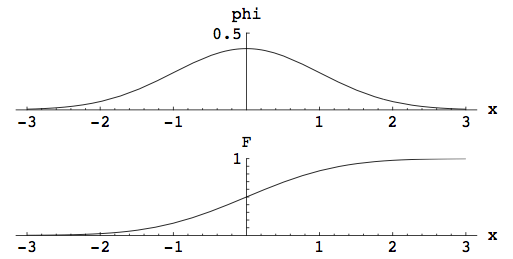
\includegraphics[width=7.5cm]{bilder/normalverteilung.png}
        Density function (above) and distribution function (below) of the normal distribution. 
        \end{minipage} \\ \\
        $ 68\% $ of the values lie within the interval $[ \mu - \sigma, \mu + \sigma]$, 
        $95\% $ in $[ \mu - 2\sigma, \mu + 2\sigma]$,    
        $99.7\% $ in $[ \mu - 3\sigma, \mu + 3\sigma]$\\\\
        \textbf{ Normal Distribution with Multiple Variables}\\
        $\varphi_{x,y}(\alpha,\beta)=\frac{1}{2\pi \sigma_x \sigma_y \sqrt{1-\rho_{xy}^2}}
            e^{-\frac{1}{2(1-\rho_{xy})^2} + \frac{(\alpha - m_x)^2}{\sigma_x^2} 
            - 2\rho_{xy}\frac{(\alpha - m_x)\beta - m_y)^2}{\sigma_x \sigma_y} + \frac{(\beta - m_y)^2}{\sigma_y^2}}$\\
            $\varphi_x(\textbf{x})=\frac{1}{(2\pi)^{\frac{n}{2}}|\textbf{C}_x|^{\frac{1}{2}}}\cdot 
            e^{-\frac{1}{2}(\textbf{x} - \textbf{m}_x)^T \textbf{C}_x^{-1} (\textbf{x} - \textbf{m}_x)}$ with \\
            $\textbf{m}_x=[E(x_1), E(x_2), \ldots, E(x_n)]^T$ and covariance matrix $\textbf{C}_x$; $c_{ij} = E((x_i-E(x_i)(x_j-E(x_j))))$ \\
        \textbf{Calculation Rule for the Normal Distribution with Multiple Variables}
        \begin{itemize}
          \item if $z=a x + b y$ then \\
          $m_z =  a m_x + b m_y$\\
          $\sigma_z^2 = a^2\sigma_x^2 + b^2\sigma_y^2+2ab\sigma_x\sigma_y$
          \item if x and y are uncorrelated, then \\
                $f_{x,y}(\alpha, \beta) = \varphi_x(\alpha)\varphi_y(\beta)$ meaning x and y are also statistically independent.
          \item The optimal nonlinear estimator for the values $\mu$ and $\sigma$ is the same as the linear estimator.
        \end{itemize}


		\subsection{Random Processes}
		\begin{minipage}{10.3cm}
			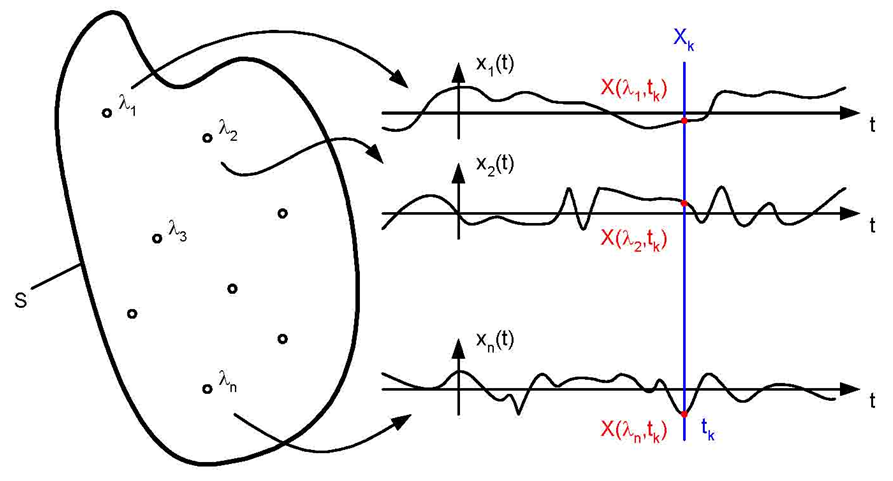
\includegraphics[width=10cm]{bilder/zufallsprozess.png}
		\end{minipage}
		\begin{minipage}{8.5cm}
			In a \textbf{random process}, each \textbf{outcome} \boldmath$\lambda$ from 
			the \textbf{outcome space} $S$ is assigned a \textbf{deterministic} \textbf{function} $x(\lambda, t)$
			\unboldmath. \\
			Random processes describe a deterministic time function triggered by the outcome of
			a random experiment. e.g., $sin(\omega t + X)$ where X is a random variable assigned from the event space at the beginning.\\
			Temporally \textbf{randomly occurring functions} can also be seen as \textbf{deterministic functions} 
			\textbf{interpreted} in such a way that the observer never knows which specific function $x_\lambda(t)$
			is present.  \\ \\
			For comparison: In the case of random variables, each elementary event is assigned a number. 
		\end{minipage} 
		\vspace{0.5cm} \\

		\subsubsection{Statistical Averages (Ensemble Averages)}
		The statistical averages are a function of time $t$, as they are averages over the
		ensemble (entire outcome space). Here, all deterministic functions are averaged at a
		specific time $t$.

		\renewcommand{\arraystretch}{1.4}
		\begin{tabular}[c]{ p{4.5cm}  p{13.5 cm}  }
			\textbf{Expected Value}:   &  $\mu_{x}(t) = E\left[X(t)\right] =
				  \int\limits_{-\infty}^{+\infty} x \cdot f_{x}(x;t)\;dx$ or $=\frac{1}{N}\sum\limits_{i=1}^{N}x_i(n)$ \\
			\textbf{Expected Value of a Deterministic Signal}:& $\mu_f(t) = E(f(t))=f(t)$\\
			\textbf{Variance}: &         $\sigma_x^2(t)=E((x(t)-\mu_x(t))^2)=c_x(t_1,t_1)$
		\end{tabular}
		\renewcommand{\arraystretch}{1}


		\subsubsection{Stationarity}
		A stationary process does not change its statistical properties over time. \\
		
		\textbf{Strict Sense Stationarity (SSS)}\\
		In a strictly stationary process, the n-dimensional probability densities remain constant over
		time. That is, the \textbf{statistical properties} and thus the probability densities are the
		\textbf{same at all times}.
		$$ f_x(x_1, x_2, \ldots, x_n; t_1, t_2, \ldots, t_n) =
				f_x(x_1, x_2, \ldots, x_n; t_1+c, t_2+c, \ldots, t_n+c) \qquad \forall (c,n \in
				\mathbb{R})$$
		
		\textbf{Wide Sense Stationarity (WSS) - Second-order Stationarity}\\
		In a weakly stationary process, the statistical properties are \textbf{not the same at every
		moment in time}, however, they are \textbf{not dependent on an absolute} point in time, but
		rather on the \textbf{difference} ($\tau$) \textbf{between two points in time} ($t_1, t_2$).  \\ 
		$$ f_x(x_1, x_2; t_1, t_2) = f_x(x_1, x_2; t_1+c, t_2+c) \qquad \forall (c \in
				\mathbb{R})$$
		\renewcommand{\arraystretch}{1.4}
		\begin{tabular}[c]{ p{3.3cm}  p{6.5cm} p{8cm} }
			\textbf{Mean}:     &  $E[X(t)] = \mu_{x} = \text{const.}$  
									& remains constant over time\\ 
			\textbf{Quadratic Mean}:    &  $E[X^{2}(t)] = r_{x}(0)$  \\ 
			\textbf{Autocorrelation}:   &   $r_{xx}(t_{1},t_{2}) = r_{x}(\tau)$
			& \multirow{2}{8cm}{only \textbf{dependent} on the \textbf{time difference} $(\tau = t_2 - t_1)$ and \textbf{not directly} on
			 the \textbf{time} $t$} \\
			 \textbf{Autocovariance}:        & $ c_{xx}(t_{1},t_{2}) = r_{x}(\tau) - \mu_{x}^{2} = c_{xx}(\tau)$ \\
		\end{tabular}
		\renewcommand{\arraystretch}{1}
		 
		A random process is always a WSS process as long as the expectation is constant and the autocorrelation function is only a function of $\tau$, i.e., both 
		statistical parameters are independent with respect to a temporal shift.    
		Every strictly stationary process is also weakly stationary, but not vice versa. 
		
		\subsubsection{Time Averages (Time Means)}
		Here, the respective deterministic functions (sample functions) are averaged over time.
		If the time average is calculated over the entire random process, then the
		time averages are \textbf{random variables}, i.e., the following two expressions are
		dependent on which function is used (hence the index $_i$).
		
		\begin{tabular}[c]{ p{4cm}  p{14.5cm}  }
			\textbf{Mean}:    &  
			$\overline{x_{i}} = \left\langle x_{i}(t) \right\rangle = 
				   \lim\limits_{T \rightarrow \infty}
					 \frac{1}{T} \int\limits_{-\frac{T}{2}}^{+\frac{T}{2}} x_{i}(t) \; dt$ \\
			   \textbf{Autocorrelation}:  &   
			$\overline{r}_{x_{i}x_{i}}(\tau) = \left\langle x_{i}(t) \cdot x_{i}(t+\tau) \right\rangle = 
				   \lim\limits_{T \rightarrow \infty}
					 \frac{1}{T} \int\limits_{-\frac{T}{2}}^{+\frac{T}{2}} x_{i}(t) \cdot x_{i}(t + \tau) \; dt$\\
			\multicolumn{2}{l}{If the \textbf{process is stationary}, the following applies: } \\
			\textbf{Mean}:    &  
			$E[\overline{x}] = 
				   \lim\limits_{T \rightarrow \infty}
					 \frac{1}{T} \int\limits_{-\frac{T}{2}}^{+\frac{T}{2}} E[x(t)] \; dt = 
					 \frac{1}{T} \int\limits_{-\frac{T}{2}}^{+\frac{T}{2}} \mu_{x} \; dt = \mu_{x}$  \\
			   \textbf{Autocorrelation}:  &   
			$E[\overline{r}_{xx}(\tau)] = 
				   \lim\limits_{T \rightarrow \infty}
					 \frac{1}{T} \int\limits_{-\frac{T}{2}}^{+\frac{T}{2}} E[x(t)x(t+\tau)] \; dt =
					 \frac{1}{T} \int\limits_{-\frac{T}{2}}^{+\frac{T}{2}} r_{xx}(\tau) \; dt = r_{xx}(\tau)$\\
		\end{tabular}
		\renewcommand{\arraystretch}{1}
		

		\subsubsection{Ergodicity}
		A stationary process is also ergodic if the \textbf{time averages} correspond to the
		\textbf{statistical averages}.
		
			\begin{minipage}{5cm}
				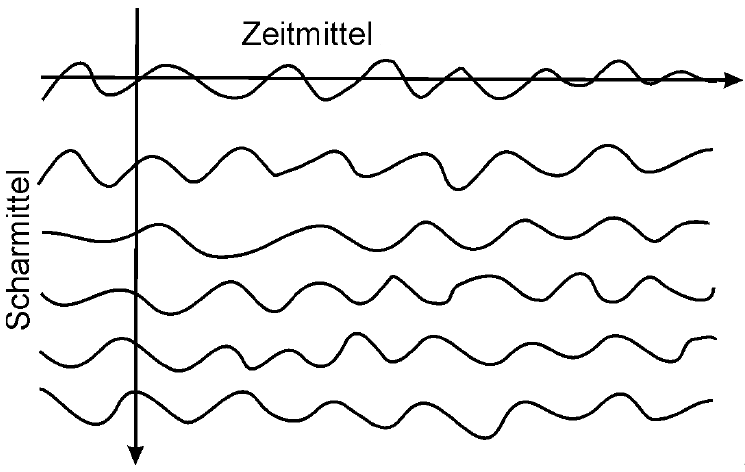
\includegraphics[width=4.5cm]{bilder/zeit-scharmittel.png}
			\end{minipage}
			\begin{minipage}{13.5cm}
		
			\begin{tabular}{ll}
				\multicolumn{2}{l}{Only in ergodic processes it necessarily holds:} \\ \\
			  $E[X(t)] = \overline{x} = \left\langle x(t) \right\rangle$ & DC-Level \\
			  $E[X(t)]^{2} = (\overline{x})^{2} = \left\langle x(t) \right\rangle^{2}$ & DC-Power \\
			  $E[X^{2}(t)] = r_{xx}(0) = \overline{x^{2}} = 
							 \left\langle x^{2}(t) \right\rangle $ & Total Power \\
			  $\sigma_{x}^{2}(t) = \left\langle x^{2}(t) \right\rangle 
								   - \left\langle x(t) \right\rangle^{2}$ & AC-Power \\
			  $\sigma_{x}(t) = \overline{\sigma}_{x}$ & RMS-Level (Effective value) of the AC signal\\
			\end{tabular} \\
			\end{minipage}
		
		
		\subsubsection{Comparison Stationary - Ergodic}
		\textbf{Swarm of mosquitoes:}\\
		\textbf{Ergodic:} If all mosquitoes fly together in a swarm, then averaged over time (Time average), each mosquito flies as fast as the entire swarm on average (Ensemble average), otherwise, the swarm could not stay together. \\
		\textbf{Stationary:} If a mosquito is sick and cannot keep up with the swarm, it flies alone and, above all, slower. Thus, its average speed (Time average) is not equal to that of the swarm (Ensemble average), so it arrives later at the destination. \\
		\textbf{Neither:} If the mosquitoes fly slower after the start, the average speed of the swarm (Ensemble average) is not constant.
		
		\textbf{School grades:}\\
		\textbf{Ergodic:} All students would have to have the same report card grade (Time average) and moreover, this grade would also have to correspond to the class average (Ensemble average) of the individual exams. \\
		\textbf{Stationary:} The class average (Ensemble average) is the same for every exam, but there are students of varying strengths with different report card grades (Time average). \\
		\textbf{Neither:} The class average (Ensemble average) is always different.
		
		\textbf{Thermal noise:} \\
		This is \textbf{ergodic} at a constant temperature.


		\subsubsection{Correlations and Power Spectra}
		Formulas in this section apply to \textbf{stationary} processes. \\
		
		\renewcommand{\arraystretch}{1.6}
		\begin{tabular}[c]{ p{3.5cm}  p{6cm} p{7.5cm} }
			\textbf{Autocorrelation}:     &  
			\multicolumn{2}{l}{$r_x(t_1,t_2)=r_x(t_1-t_2)=r_x(\tau)=r_{xx}(\tau) = E[X(t)X(t+\tau)]$} \\
			  &    $\mid \! r_{xx}(\tau) \! \mid \leq r_{xx}(0) = E[X^{2}(t)]$ 
			& $r_{xx}(-\tau) = r_{xx}(\tau) \quad$ (even, Fourier transform becomes real)\\
		  \textbf{Cross-correlation}:&     
			$r_{xy}(\tau)=r_{xy}(\tau) = E[X(t)Y(t+\tau)]$  
			& $r_{xy}(-\tau) = r_{yx}(\tau) \quad$ (Order of indices!) \\
			& $|r_{xy}(\tau)| \leq \frac{1}{2} \left[ r_{xx}(0)+r_{yy}(0)\right] $
			& $|r_{xy}(\tau)|  \leq \sqrt{r_{xx}(0)r_{yy}(0)}$ \\
		   \textbf{Autocovariance }:     &  \multicolumn{2}{l}{$c_{xx}(t_{1},t_{2}) =
				  E\left[ \left( X(t_{1})-\mu_{x}(t_{1})\right) \cdot
						  \left( X(t_{2})-\mu_{x}(t_{2})\right) \right] =
				  r_{xx}(t_{1},t_{2}) - \mu_{x}(t_{1}) \cdot \mu_{x}(t_{2})=$}\\    
			&\multicolumn{2}{l}{$c_x(\tau)=c_{xx}(\tau) = E\!\left[ \left( X(t)      - E[X(t)]      \right) \cdot
										  \left( X(t+\tau) - E[X(t+\tau)] \right) \right] =
								r_{xx}(\tau) - \mu^{2}_{x} $} \\
			\textbf{Cross-covariance}:     & \multicolumn{2}{l} {$c_{xy}(t_{1},t_{2}) = 
				  E\left[ \left( X(t_{1})-\mu_{x}(t_{1})\right) \cdot
						  \left( Y(t_{2})-\mu_{y}(t_{2})\right)^* \right] =
				  r_{xy}(t_{1},t_{2}) - \mu_{x}(t_{1}) \cdot \mu_{y}(t_{2})=$}\\    
			&\multicolumn{2}{l}{$c_{xy}(\tau) = E\!\left[ \left( X(t)      - E[X(t)]      \right) \cdot
										  \left( Y(t+\tau) - E[Y(t+\tau)] \right) \right] =
								r_{xy}(\tau) - \mu_{x}\mu_{y} $}\\
			& \multicolumn{2}{l}{Random processes are considered \textbf{uncorrelated} if $c_{xy}(\tau) = 0$}
		\end{tabular}
		\renewcommand{\arraystretch}{1}
		
		\textbf{Spectral Power}\\
		The autocorrelation function $r_{xx}(\tau)$ and power spectral density $P_{xx}(\omega)$ form a
		Fourier-\textbf{transform pair}. \\ The power spectral density can be interpreted as the \textbf{average power per frequency band} and is
		defined as follows:                             
				$$ P_{xx}(\omega) = E\left[ \lim\limits_{T \rightarrow \infty}
											\frac{1}{T} \cdot \mid\! X(\omega) \!\mid^{2}\right]                          
									= \int\limits_{-\infty}^{+\infty} r_{xx}(\tau) \cdot e^{-j\omega\tau} \; d\tau 
									\qquad \IFT \qquad
				r_{xx}(\tau)   = \frac{1}{2\pi} \int\limits_{-\infty}^{+\infty} 
									 P_{xx}(\omega) \cdot e^{j\omega\tau} \; d\omega$$ 
				or:
				 
				$$P_{xx}(z) = \sum\limits_{k=-\infty}^{\infty} r_{xx}(k)z^{-k}\qquad \IFT \qquad 
				r_{xx}(k)=\frac 1{2\pi} \int \limits_{-\pi}^{\pi} P_{xx}(e^{jw})e^{jkw}dw \qquad 
				r_{xx}(0) =\frac 1{2\pi} \int \limits_{-\pi}^{\pi} P_{xx}(e^{jw})dw = \lim\limits_{z \rightarrow 0} P_{xx}(z)$$
									 
		$P_{xx}(\omega)$ is purely real, symmetric $(P_{xx}(z)=P_{xx}^*(\frac{1}{z^*}))$ and $\geq 0$. \\
		Cross-correlations ($r_{yx}(\tau), r_{xy}(\tau)$) and cross-spectral densities ($P_{yx}(\tau),
		P_{xy}(\tau)$) form a Fourier-transform pair.
		\begin{center}
		$ r_{yx}(\tau) \FT P_{yx}(\omega) \qquad \qquad r_{xy}(\tau) \FT P_{xy}(\omega)  $
		\end{center}
		Since autocorrelations are definitely non-causal (defined also for negative time values), the bilateral z-transform must be applied.
		
		The eigenvalues of the autocorrelation matrix have the following limitation:\\
		$$\min\limits_\omega P_{xx}(z)\leq \lambda_i \leq \max\limits_{\omega}P_{xx}(z)$$
		

		\subsubsection{Autocorrelation Examples}
		\begin{tabular}{|l|l|l|}
			\hline
				White Noise
				& $r_{xx} (n) = \frac {N_0}{2} \delta(n) \FT P_{xx}(z)= \frac {N_0}{2};\hspace{0.25cm}$ & all z\\
			\hline
				First-Order Process
				& $r_{xx} (n) = P_s \cdot a^{|n|} \FT P_{xx} (z) = P_s \cdot \frac {1-a^2}{(1-az^{-1})(1-az)}$ & for $a<|z| < \frac{1}{a}$\\
			\hline
				
				& $r_{xx} (n) = a^n(u(n) - u(n-N)) \FT P_{xx} (z) = \frac{1-a^Nz^{-N}}{1-az^{-1}}$ & for $|z| > 0$\\
			\hline
				
				& $r_{xx} (n) = a^n \cdot u(n) \FT P_{xx} (z) = \frac{1}{1-az^{-1}}$ & for $|z| > a$\\
			\hline
				
				& $r_{xx} (n) = -a^n \cdot u(-n-1) \FT P_{xx} (z) = \frac{1}{1-az^{-1}}$ & for $|z| < a$\\
			\hline
				Binary Data Signal
				& $r_{xx} (0) = P_s = A_1^2p_1 + A_0^2 p_0 $ &\\
				&$r_{ss} (|n| < T) = $ linear transition from $r_{ss}(0)$ to $r_{ss} (|n| = T)$ &\\
				& $r_{xx} (|n| \geq T) = P_s = A_1^2p_1^2 + A_0A_1p_0p_1 + A_1A_0p_1p_0 + A_0^2p_0^2$ &  \\
			\hline
				Superimposed Signals
				& $r_{gg\pm}(n) = r_{ss}(n) + r_{sf}(n) + r_{sf}(-n) + r_{ff}(n) $ &\\
				$g_\pm(t) = s(t) \pm f(t)$
				&  $\FT P_{g+}(\omega) = P_{s}(\omega) + P_{f}(\omega) \pm 2 \text{Re} \{P_{sf}(\omega) \}$ &\\ 
			\hline
		\end{tabular} 
		\vspace{-0.5cm}
		\subsubsection{Numerical Calculation}
		\begin{tabular}{|l|l|}
			\hline
				\multicolumn{2}{|l|}{\textbf{Numerical Calculation}} \\
			\hline
			Autocorrelation
				& $\hat{r}_{xx} (n) = \frac 1 N \sum\limits_{m=0}^{N-1} s(m ) s[(m+n) ] 
											 = \frac 1 N \sum\limits_{m=0}^{N-1} s[(m-n) ] s(m ) \DFT \hat{P}_{xx}(z)$ \\
			\hline
			Cross-correlation
				& $\hat{r}_{xy} (n ) = \frac 1 N \sum\limits_{m=0}^{N-1} s(m ) f[(m+n) ] 
											 = \frac 1 N \sum\limits_{m=0}^{N-1} s[(m-n) ] f(m ) \DFT \hat{P}_{xy}(z) $ \\
			\hline
			Power Spectral Density 
				& $\hat{P}_{xx}(z) = \frac 1N \left|S_T(z)\right|^2 \IDFT \hat{r}_{xx} (n )
					\qquad \text{with} \quad S_T(z) \IDFT s(n)$\\
			\hline
			Cross Power Spectral Density 
				& $\hat{P}_{xy}(z) = \frac 1N S_T^*(z) F_T(z) \IDFT \hat{r}_{xy} (n )
				\qquad \text{with} \quad F_T(z) \IDFT f(n)$\\

			\hline
		\end{tabular}


		\subsubsection{Transmission of Random Processes through LTI Systems}
		A random process is transmitted through an LTI system. \hspace{2cm} $Y(t) = L[X(t)] \Rightarrow
		Y(t) = h(t) \ast X(t)$ \vspace{0.3cm}\\
		\renewcommand{\arraystretch}{1.4}
		 \begin{tabular}[c]{ p{2cm}  p{8.5cm} p{8cm} }
			& \textbf{General} & \textbf{WSS Process} \\
			\textbf{Mean}
				& $\mu_{y}(t) = h(t) \ast \mu_{x}(t)$
				& $\mu_{y} = H(0) \mu_{x}$ \\
			\textbf{Autocorrelation\textcolor{red}{*}}
				& {$r_{yy}(t_{1},t_{2}) = \int\limits_{-\infty}^{+\infty}
				\int\limits_{-\infty}^{+\infty} h(\alpha) h(\beta)
							  r_{xx}(t_{1}-\alpha, t_{2}-\beta) \; d\alpha \; d\beta$}
				& {$r_{yy}(\tau) = \int\limits_{-\infty}^{+\infty}
				\int\limits_{-\infty}^{+\infty} h(\alpha) h(\beta)
							  r_{xx}(\tau+\alpha-\beta) \; d\alpha \; d\beta$} \\
			\textbf{Spectral Power}
				&
				& $P_{yy}(\omega)= H^{\ast}(\omega) H(\omega) P_{xx}(\omega)
					= |H(\omega)|^{2} P_{xx}(\omega)$  \\
		\end{tabular}
		\renewcommand{\arraystretch}{1} \\
		\textcolor{red}{*} = It is much simpler to calculate the autocorrelation from the spectral power
		(transform pair) - instead of from this dreadful integral. \\
		A WSS process at the input also produces a WSS process at the output.
		
		\subsubsection{Filtering of Random Processes}
		The output autocorrelation $r_y(k)$ is\\
		 $r_y(k) = r_x(k)\ast h(k) \ast h^*(-k)$ or $\boxed{P_{y}(z) = P_{x}(z)\cdot H(z) \cdot H^*(\frac{1}{z^*}) \quad
		  P_{y}(e^{j\omega})=P_x(e^{j\omega})\cdot|H(e^{j\omega})|^2}$
		
		\subsubsection{White Noise}
		\begin{center}
			\begin{minipage}{8cm}
				$P_{xx}(\omega) = \dfrac{\eta}{2} \qquad r_{xx}(\tau) = \dfrac{\eta}{2} \cdot \delta(\tau)= \sigma_x^2 \cdot \delta(\tau)$ \\ \\
				Example: thermal noise of resistors \\
				\textbf{Decreases} in practice in the \textbf{Tera-Hz range}!
			\end{minipage}
			\begin{minipage}{10cm}
				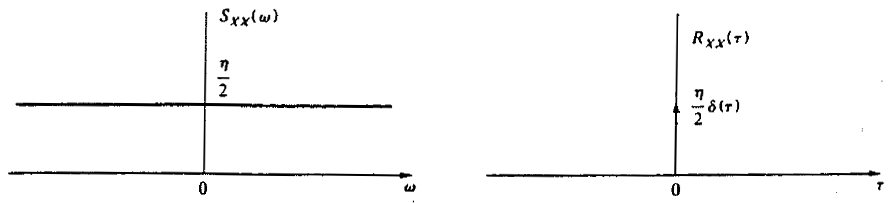
\includegraphics[width=9cm]{bilder/weisses_rauschen.png}
			\end{minipage}
		\end{center}


		\subsubsection{Colored Noise Signals}
		\renewcommand{\arraystretch}{2}
		\begin{tabular}[c]{ | p{4cm} | p{3.5cm} | p{3cm} | p{6cm} | }
			\hline
				\textbf{Term (German)}
				& \textbf{Term (English)}
				& \textbf{Power Spectrum}
				& \textbf{Note} \\
			\hline
				Rosa Rauschen
				& Pink Noise
				& $P_{xx}(\omega) = c \cdot \dfrac{1}{\omega}$
				& Test signal for audio engineering, due to constant power per octave \\
			\hline
				Braunes/Rotes Rauschen
				& Brown/Red Noise
				&   $P_{xx}(\omega) = c \cdot \dfrac{1}{\omega^2}$
				& \\
			\hline
				Blaues Rauschen
				& Blue Noise
				&   $P_{xx}(\omega) = c \cdot \omega$
				& \\
			\hline
				Violettes Rauschen
				& Purple/Violet Noise
				&   $P_{xx}(\omega) = c \cdot \omega^2$
				& \\
			\hline
		\end{tabular}
		\renewcommand{\arraystretch}{1}


\subsection{Estimation \hayes{72}}
  \subsubsection{Bias}
    The bias is the difference between the real value $\Theta$ and the estimate $\hat{\Theta}$: 
    $B = \Theta - E(\hat{\Theta}_N)$. When $B=0$, the estimator is \em unbiased\em. When the estimator
    is biased but the bias goes to zero as the number of observations $N$ goes to infinity, then
    the estimator is \em asymptotically unbiased \em ($\lim_{N \rightarrow \infty} E(\hat{\Theta}_N) = \Theta$). 
    If the bias stays $B \neq 0$, the estimator is \em biased\em.
    
  \subsubsection{Consistency}
    If $\lim_{N \rightarrow \infty} Var(\hat{\Theta}_N) = 0$, the estimator is consistent. 
    $\hat{\Theta}_N$ is said to \em converge to $\Theta$ with probability one\em. 
    Here, a \em consistent \em estimator if it is asymptotically unbiased and has a variance that
    goes to zero as $N$ goes to infinity.
     
